\chapter{Classification}

Classification is a type of supervised learning. The data needed for classification is a set of instances, where each instance is a tuple $<x,y>$, where $x$ is the set of attribute value that describe the instance, and $y$ is the \textbf{class label} of the instance. The values of $x$ can be of any type, while the class label must always be categorical. If the target is not categorical, then the task is a regression task.

\section{General Framework}

The goal of a classification task is to produce a \textbf{model} (classifier) that correctly predicts the output on any input data. The model is created on the basis of a set of instances called \textbf{training set (TR)}, and through a \textbf{learning algorithm}, the model can be adapted to the training data using \textbf{induction}. Afterwards, the model can be applied on unseen data to perform \textbf{deduction}. To estimate the performance of the final model, a \textbf{test set (TS)} is used, which is composed of never-seen-before instances.

\section{K-NN (K-Nearest Neighbors)}

(SEE ML NOTES)

A K-NN learner is a type of instance based/lazy classifier. This learner represents each instance in the training set as a point in a n-dimensional space. The data is simply stored as is, and for each new instance provided as input, its class/value is estimated by looking at the label of the k points closest to it. 

If it's a classification task, the output will correspond to the majority vote. If there's two classes, the output is calculated as:
\begin{equation*}
    h(x) = \begin{cases}
        1 & \textit{avg}_k(x) > 0.5 \\
        0 & \text{else}
    \end{cases} \, ,
\end{equation*}
Or, in the case of multiple classes:
\begin{equation*}
    h(x) = \arg \max_v \sum_{x_i \in N_k(x)} 1_{v,y_i}  \, ,
\end{equation*}
\begin{equation*}
    1_{v,y_i} = \begin{cases}
        1 & v = y_i \\
        0 & else
    \end{cases}
\end{equation*}
If it's a regression task, it will be calculated as the mean of the labels:
\begin{equation*}
    h(x) = \textit{avg}_k(x) = \frac{\sum_{x_i \in N_k(x)} y_i}{k}
\end{equation*}

K-NN is not a model in the traditional sense; it does not produce an hypothesis that can be used on any new input, and instead constructs a new hypothesis \textit{ad hoc} for each input.

A key aspect to consider when using K-NN is setting the appropriate value of $k$. If $k$ is too big, for example $k$ close to $l$ (the number of training instances), then it will perform poorly, since each input, including training points, will always correspond to the same output (majority vote among all points/mean of all labels), thus leading to underfitting. If $k$ is instead too small, for example $k = 1$, then we will have overfitting, where each training point is classified correctly, but we will have high generalization error for unseen data, since the output will be estimated by looking at the single closest point to it. As a general practice, $k$ is set to $\sqrt{l}$, although the method is not infallible.

A variant of K-NN uses weighted voting, were weights are calculated as the inverse of the distance between the input and the neighbor so that closer points will influence the result much more than distant ones. The hypothesis for classification becomes:
\begin{equation*}
    h(x) = \arg \max_v \sum_{x_i \in N_k(x)}  \dfrac{1_{v,y_i}}{d(x,x_i)^2} \, ,
\end{equation*}
while the one for regression becomes:
\begin{equation*}
    h(x) = \frac{1}{k}\sum_{x_i \in N_k(x)} \dfrac{y_i}{d(x,x_i)^2} \, .
\end{equation*}

The main issue of K-NN is that it's susceptible to the curse of dimensionality: as the number of dimensions in the data increases, the density of the points decreases, therefore estimation of new inputs will be less and less accurate as it won't be as local anymore. K-NN is also sensitive to scaling, since it deals with distances.

The main advantages of K-NN are that it's very simple to implement, and can be easily "retrained" by adding or removing instances. It can also create decision boundaries of any shape. The main disadvantages are (other than the ones explained above) that since it's a lazy learner, it needs all the data to be available to make an estimation, so it's very demanding in terms of space needed, as well as computational time, since estimating an output has a complexity of $O(ln)$ (where $l$ is the number of instances and $n$ is the number of dimensions). It also does not handle missing values.

\subsection{Parallel Exemplar-Based Learning System (PEBLS)}

PEBLS is a 1-NN system that can be used for categorical attributes as well as numeric ones. For categorical attributes, the distance is calculated as follows:

\begin{equation*}
    d(V_1,V_2) = \sum_i | \dfrac{n_{1_i}}{n_1} - \dfrac{n_{2_i}}{n_2} | \, ,
\end{equation*}
where $V_1$ and $V_2$ are two values of the same attribute, $n_1$ and $n_2$ are the number of times values $V_1$ and $V_2$ respectively appear in the dataset, and $n_{1_i}, n_{2_i}$ are the amount of times that $n_1$ and $n_2$ respectively correspond to the target label $i$.

The distance between two records $X$ and $Y$ is calculated as:

\begin{equation*}
    \delta (X, Y) = w_X w_y \sum_i d(X_i, Y_i) \, ,
\end{equation*}
where $w_X$ and $w_Y$ are weight assigned to the records. Each weight is calculated as:
\begin{equation*}
    w_Z = \dfrac{N_{Z_{\textit{predict}}}}{N_{Z_{\textit{correct}}}} \, ,
\end{equation*}
so it's the ratio between the amount of times the record $Z$ is used for prediction and the amount of times the prediction using $Z$ is actually correct. The less a record is reliable for prediction, the higher its weight and therefore distance from other records.

The algorithm then operates like a normal 1-NN.

\section{Naïve Bayes Classifier}

A Naïve Bayes Classifier is one of the simplest probabilistic classification models. This class of models make use of probability theory to estimate values of inputs.

Before delving into the details of the algorithm, let's see some basic probability theory:

\begin{itemize}
    \item $P$ is a probability function, going from 0 to 1.
    \item $X=x$ is an event. $P(X=x)$ is the probability of said event happening.
    \item The \textbf{joint probability} of two events, $P(X=x, Y=y)$, calculates the probability that $X=x$ and $Y=y$ both happen together. If they're independent, then $P(X=x, Y=y) = P(X=x) * P(Y=y)$.
    \item The \textbf{conditional probability} of two events, $P(Y=y|X=x)$, calculates the probability that $Y=y$ given that $X=x$ already happened.
    \item The joint probability can be calculated using conditional probability and vice versa: $P(X=x,Y=y) = P(Y=y|X=x) * P(X=x) = P(X=x|Y=y) * P(Y=y)$.
    \item \textbf{Bayes theorem} states that:
    \begin{equation*}
    P(Y=y|X=x) = \dfrac{P(X=x,Y=y)}{P(X)} = \dfrac{P(X=x|Y=y) * P(Y)}{P(X)}.
    \end{equation*}
    \item Another useful property is that $P(X=x) = P(X=x, Y=0) + P(X=x, Y=1)$.
\end{itemize}

In the context of this classifier, the different terms of the joint probability $P(Y=y|X=x)$ have specific names:

\begin{table}[h]
    \centering
    \begin{tabular}{c|c}
        $P(Y=y|X=x)$ & Posterior probability\\
        $P(X=x|Y=y)$ & Likelihood \\
        $P(Y)$ & Prior probability \\
        $P(X)$ & Evidence \\
    \end{tabular}
\end{table}

The learning algorithm can find the posterior probability for any possible couple of events $X$ and $Y$; a new record $X'$ can be classified by finding the class $Y'$ that maximizes the posterior probability $P(Y'=y'|X'=x')$. This estimation is always done under the \textbf{Naïve Bayes Assumption}: all the attributes are \textbf{conditionally independent} of each other given a class label $y$, that is:

\begin{equation*}
    P(X=x|Y=y) = \prod_i P(X_i = x_i|Y=y) \, ,
\end{equation*}
where each $X_i$ is a different attribute of the record $X$. In practice, this means that the attributes are only influenced by the target class, and if we know the class label, the attributes are independent of each other. In general, given three variables $X_1$, $X_2$, and $Y$, we say that $X_1$ is conditionally independent of $X_2$ given $Y$ if:

\begin{equation*}
    P(X_1 | X_2,Y) = P(X_1|Y) \, .
\end{equation*}

Because of this assumption, the conditional probability $P(X_i | Y)$ can be calculated for each possible attribute/class value pair, and those same probabilities can be multiplied to calculate the probability for a whole record. Obviously, we don't actually know the ``real'', ground-truth probability of the variables, so we must make some estimations based on the available data.

For categorical data, we calculate $P(Y=y) = \frac{N_y}{N}$, i.e., it's the ratio between the number of records with label $y$ and the overall number of records, and $P(X=x|Y=y) = \frac{N_{xy}}{N_y}$, so the number of times a record has value $x$ for the attribute $X$ and the target label is $y$, divided by the number of total records with label $y$.

Consider the dataset described by the table below.
\begin{figure}[h]
    \centering
    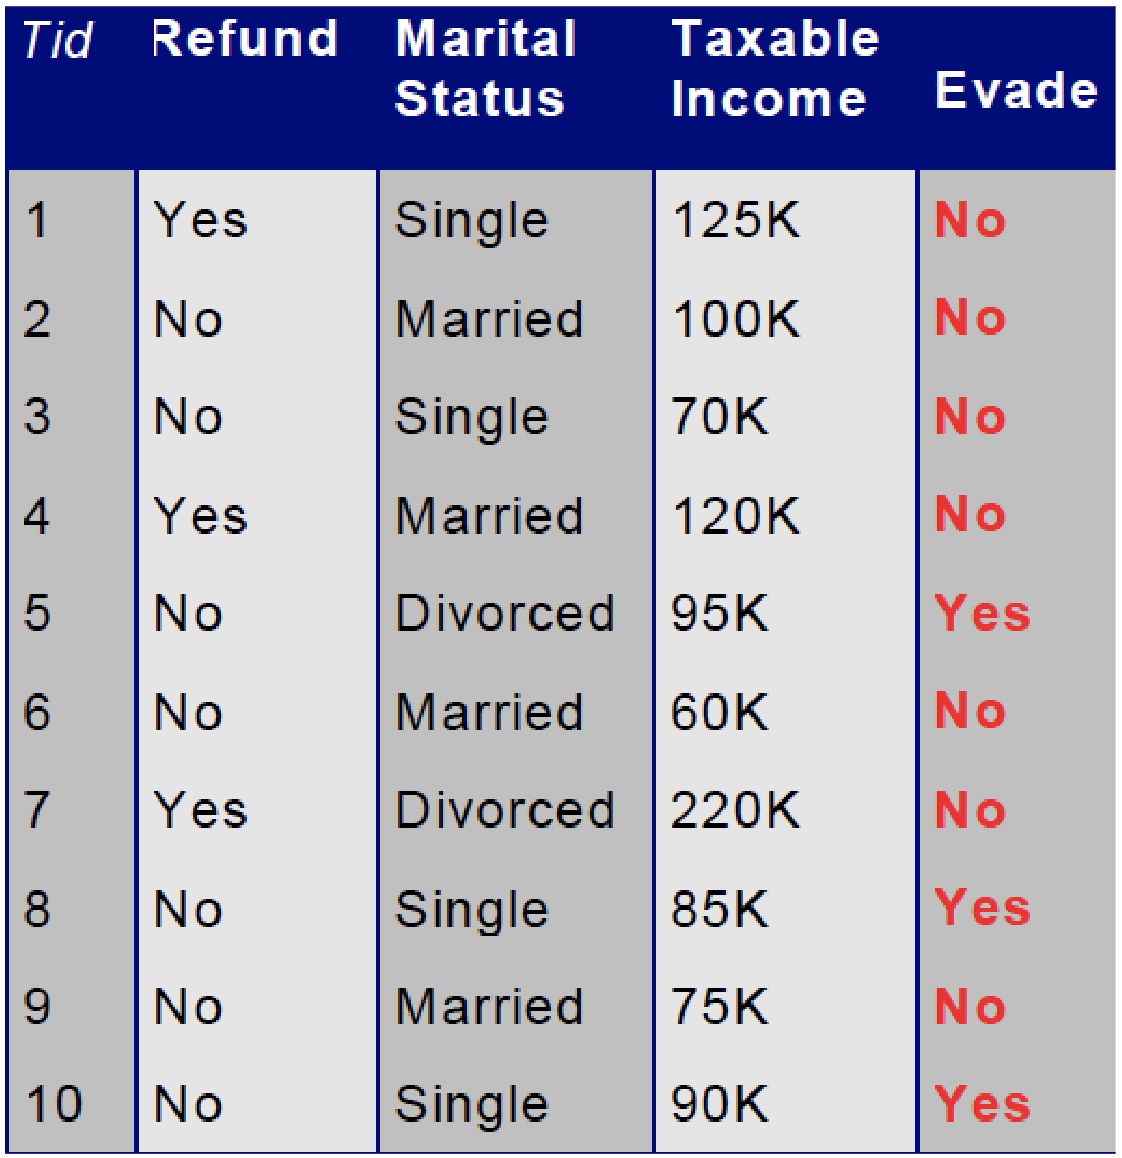
\includegraphics[width=0.5\linewidth]{img/NBC.png} 
\end{figure}

Then, $P(\textit{Evade} = \textit{Yes}) = 3/10$, and $P(\textit{Marital\_Status} = \textit{Single} | \textit{Evade} = \textit{Yes}) = 2/3$.

Datasets, however, often contain continuous data. In order to deal with such attributes, the solutions can be:
\begin{itemize}
    \item Discretization of the values into bins, although it would violate the independence assumption;
    \item Two way split, so the values are split into two intervals and we choose one of them, although this approach may lose information;
    \item We use a \textbf{probability density distribution}. This means that we assume a certain distribution function for the variable and use it on unseen data.
\end{itemize}

A commonly used distribution function is the \textbf{Gaussian/normal distribution function}:

\begin{equation*}
    P(X_i = x_i | Y = y_j) = \dfrac{1}{\sqrt{2 \pi} \sigma_{ij}} e^{-\frac{(x_{ij} - \mu_{ij})^2}{2 \sigma_{ij}^2}} \, ,
\end{equation*}
where the mean $\mu_{ij}$ can be estimated as the mean of $X_i$ for all the records belonging to class $y$, and the variance $\sigma_{ij}^2$ can be estimated as the sample variance $s^2$ of the same records.

One thing to notice is that if the conditional probability for any attribute is 0, then the likelihood will be 0 as well. Zero conditional probabilities arise then the number of training instances is small and the number of possible values of an attribute is large. The Naïve Bayes Classifier, as is, cannot classify records when this happens. To address the problem, it is important to adjust the conditional probability estimates so that they are not simple fractions of training instances. This can be achieved by using the following alternate estimates of conditional probability:

\begin{equation*}
    P(X = x| Y = y) = \dfrac{N_{xy} + 1}{N_y + |Y|} \, \text{(\textbf{Laplace estimate})},
\end{equation*}

\begin{equation*}
    P(X = x| Y = y) = \dfrac{N_{xy} + mp}{N_y + m} \, \text{(\textbf{M-estimate)}}.
\end{equation*}
Here, $v$ is the total number of attribute values that $X$ can take. $p$ is an initial estimate of $P(X = x | y)$ that is known a priori, and $m$ is an hyperparameter that represents our confidence in using $p$ when the fraction of training examples is too brittle. Note that these estimates provide non-zero values even when $n_c = 0$.

Summing up, Naïve Bayes Classifiers:
\begin{itemize}
    \item are robust to isolated noise points since they don't significantly influence the conditional probability estimates;
    \item can easily compute probabilities even in high-dimensional spaces, provided attributes are actually conditionally independent of each other giver the class labels;
    \item can handle missing values in both training and test instances, by simply ignoring them.
    \item are robust to irrelevant attributes, because if $X$ is an irrelevant attribute, then $P(X=x|Y=y)$ becomes almost uniformly distributed.
\end{itemize}
In case the Naïve Bayes Assumption does not hold, we need to use different frameworks, such as Bayesian Networks.

\section{Decision Tree Classifier}

To illustrate how a decision tree works, we will use a practical example. Imagine a classification problem in which the data is represented by vertebrate animals, and the target is to distinguish them into mammals and non-mammals. One approach to solve the classification problem is to pose a series of questions about the characteristics of the animal. Is it cold-blooded? If yes, it's a reptile. Otherwise, does it have feathers? Again, if yes, it's a bird. So, if it's warm-blooded and has no feathers, it's a mammal.

In general, we can ask a series of questions about the attributes of the instance, and for each answer we receive, we can either give a verdict or ask a new question, until the instance is classified. The questions and answers can be organized in a \textbf{decision tree}. A decision tree has three types of nodes:
\begin{itemize}
    \item A \textbf{root node}, with no incoming links and $l \in \mathbb{N}$ outgoing links;
    \item \textbf{Internal nodes}, each with one incoming link and $l \in \mathbb{N} \setminus \{0,1\}$ outgoing links;
    \item \textbf{Leaf/terminal nodes}, each with one incoming link and 0 outgoing links.
\end{itemize}
Every leaf is associated with a class label, while the internal nodes are associated to an attribute test condition, typically defined using only one attribute at a time. Each possible outcome is associated with a child of the node.

Given a decision tree, classifying an unseen instance is straightforward: starting from the root, choose the child that corresponds to the answer of the attribute test, and stop once a leaf node is reached. The outcome in the leaf node will be the output of the model on that instance. By constructing a decision tree for the previous animal example, if we were to classify the following instance:
\begin{table}[h!]
    \centering
    \begin{tabular}{c|c|c}
        name & coldBlood & feathers \\
        \hline
        owl & no & yes \\
    \end{tabular}
\end{table}

we would answer "no" and "yes" to the first two questions, thus classifying it as a non-mammal. But how is the decision tree built?

\subsection{Decision Tree Induction}

There's a few different algorithms that can build decision trees. One of the earliest ones is \textbf{Hunt's algorithm}, which is also the basis for more recent ones such as \textbf{ID3}, \textbf{C4.5}, and \textbf{CART}.

\subsubsection{Hunt's algorithm}

In this algorithm, the decision tree is built recursively. The tree initially contains only one node, the root, associated with all the training instances. If it's associated with instances belonging to multiple classes, it is expanded using an attribute test condition determined through a \textbf{splitting criterion}. A child leaf node is constructed for all possible outcomes of the test, and the instances of the father are distributed among them. This expansion is repeated recursively on all leaves, until a leaf can no longer be expanded since it represents only one class label.

This algorithm makes some simplifying assumptions that are often not true in practice:
\begin{itemize}
    \item Some of the child nodes may be empty if none of the training examples have the particular attribute values; one way to handle this is to declare each of them as a leaf node with a class label that occurs most frequently among the training instances associated with the parent node.

    \item If all training instances associated with a node have identical values, it's not possible to expand the node. One way to handle the problem is to declare the node as a leaf and assign it to the class label that occurs most frequently in it.
\end{itemize}

\subsubsection{ID3, C4.5, CART}

ID3 uses Hunt's algorithm with information gain criterion and gain ratio. C4.5 improves ID3, but needs all the data to fit in memory, can handle missing values for continuous attributes, performs tree post-pruning, and is unsuitable for large datasets. CART builds multivariate decision binary trees.

\subsection{Design Issues In Tree Induction}

Hunt's algorithm is a generic procedure for growing decision trees in a greedy fashion. To implement the algorithm, there are two key design issues to address:

\begin{itemize}
    \item \textbf{The splitting criterion}, so which attribute to select at each iteration to partition the dataset, and how should the instances be distributed to child nodes.

    \item \textbf{The stopping criterion}, so when expanding of nodes should stop. Obviously, if we run the algorithm with no restrictions, it will eventually only find unsplittable leaf nodes and terminates. However, we may still choose to interrupt the splitting on nodes even if they contain instances of more than one class to avoid overfitting of the training data, using a regularization technique called \textbf{early termination/early stopping}.
\end{itemize}

\subsection{Methods for Expressing Attribute Test Conditions}

Induction algorithms must provide a method for expressing an attribute test condition and corresponding outcomes for different attribute types.

For \textbf{binary attributes}, the test condition will generate two possible outcomes. For \textbf{nominal attributes}, which may have multiple values, the attribute test condition can be expressed either as a binary split, isolating one or more value from all the rest, or a multiway split, with one new node for each value. For \textbf{ordinal attributes}, the attribute test condition can also produce either a binary or multiway split, but the grouping in the binary one must respect the order property of the values. For \textbf{continuous attributes}, the attribute test condition can be expressed as a comparison test producing a binary split, or a range query through discretization producing a multiway split. In this last case, discretization may be static (the values are discretized once at the beginning), or dynamic (the discretization is repeated at each node).

\subsection{Methods for Selecting an Attribute Test Condition}

There are many measures that can be used to determine the goodness of an attribute test condition. These measures try to give preference to attribute test conditions that partition the instances into purer subsets in the child nodes, which means that each child contains instances belonging mostly to one class. Having a purer subset means that the corresponding node will be expanded less (or not at all, if it contains only one class), while having impure subsets may require a lot of splits and therefore a deeper tree, which might be susceptible to overfitting.

The idea is to calculate the \textbf{impurity} of a node through an appropriate measure, both before and after splitting, and to choose the attribute test condition that produces the highest $\textit{Gain} = \textit{Impurity}_{\textit{pre}} - \textit{Impurity}_{\textit{post}}$ (or, equivalently, the lowest impurity measure after splitting). The following are some commonly used impurity measures; $p_i(t)$ refers to the relative frequency of training instances that belong to class $i$ at node $t$, and $c$ is the total number of classes.

\BoxDef{Gini Index}{
\begin{equation*}
   \textit{Gini} = 1 - \sum_{i=0}^{c-1} p_i(t)^2
\end{equation*}
Maximum: $1-1/c$ \hfill Minimum: $0.0$
}
The Gini Index for a collection of nodes is calculated as:
\begin{equation*}
    \textit{Gini}_{\textit{split}} = \sum_{i=1}^k \dfrac{n_i}{n} \textit{Gini}(i) \,,
\end{equation*}
where $n_i$ is the number of records at child $i$ and $n$ is the number of records at parent node $p$. To choose the attribute for the current split to perform, we select the one that minimizes the weighted average Gini index of the children.

For categorical attributes, the count matrix is calculated considering each distinct value, and an index is produced for the different possible multiway/binary splits.

For continuous attributes, the construction of the count matrix is not as immediate. The split is done by choosing one or more threshold values to separate instances based on a inequality test: for a basic binary split, a value $v$ must be chosen so that one child node will contain all instances with $\textit{attr} \leq v$, and the other child node will contain all instances with $\textit{attr} > v$. The bruteforce approach to find the idea value of $v$ is to pick one value of the attribute at a time to use as a threshold, scan the database to compute the count matrix, and determine the Gini index. This approach is obviously inefficient, with a complexity of $O(n^2)$ (where $n$ is the number of training instances).

A more efficient algorithm is the following:
\begin{enumerate}
    \item the instances are sorted by value of the attribute;

    \item the split positions are calculated as the midpoints between every couple of adjacent sorted values;

    \item the new splits are linearly scanned updating each time the count matrix and Gini index;

    \item the split position is chosen as the one with the lowest index.
\end{enumerate}
This algorithm has a complexity of $O(nlog(n))$.

\BoxDef{Entropy}{
\begin{equation*}
    \textit{Entropy} = - \sum_{i=0}^{c-1} p_i(t) \log_2 (p_i(t))
\end{equation*}
Maximum: $\log_2(c)$ \hfill Minimum: $0.0$
}

The entropy is used the same way as the Gini index: the lower the value, the better the split.

\BoxDef{Classification Error}{
\begin{equation*}
    \textit{Classification error} = 1 - \max_i p_i(t)
\end{equation*}
Maximum: $1-1/c$ \hfill Minimum: $0.0$
}

Overall, all three measures are coherent with each other, but may lead to different choices in terms of what attributes to use for the split. 

\subsubsection{Gain Ratio}

One limitation of impurity measures is that the tend to favor qualitative attributes with large number of distinct values. Having a low impurity value alone is not enough to find a good attribute test condition for a node. There are two ways to overcome this problem: one way is to generate only binary decision trees, avoiding the problem of handling attributes with varying values altogether. Another way is to modify the splitting criterion to consider the number of partitions produced by the attribute as well.

In the C4.5 algorithm, a measure known as \textbf{gain ratio} is used, which compensates for attributes that produce a large number of child nodes.

\BoxDef{Gain ratio}{
The gain ratio is calculated as:
\begin{equation*}
    \textit{Gain ratio} = \dfrac{\textit{Gain}}{\textit{Split info}} = \dfrac{\textit{Entropy}(p) - \sum_{i=1}^k \dfrac{N(v_i)}{N} \textit{Entropy}(v_i)}{- \sum_{i=1}^k \dfrac{N(v_i)}{N} \log_2(\dfrac{N(v_i)}{N})}
\end{equation*}
where $N(v_i)$ is the number of instances assigned to node $v_i$, and $k$ is the total number of splits.
}

\subsection{Algorithm for Decision Tree Induction}

We can now present a full pseudocode for a decision tree induction algorithm.

\begin{algorithm}
\caption{Pseudocode for a decision tree induction algorithm.}
\texttt{TreeGrowth}$(E,F)$
\begin{algorithmic}[1]
        \If{\texttt{stopping\_cond}$(E,F)$}
            \State leaf = \texttt{create\_node()}
            \State leaf.label = \texttt{classify}$(E)$
            \State return leaf
        \Else
            \State root = \texttt{create\_node()}
            \State \textit{root.testcond} = \texttt{find\_best\_split}$(E,F)$

            \For{$v \in $ root.testcond.outcome}
                \State $E_v$ = $\{e | \textit{root.testcond}(e) = v \land e \in E \}$
                \State child = \texttt{TreeGrowth}$(E_v,F)$
                \State add child as descendant to root and label the edge as $v$.
            \EndFor
        \EndIf
        \State return root.
\end{algorithmic}
\end{algorithm}

\subsection{Advantages of Decision Tree Classifiers}

The following is a summary of the most important characteristics of decision trees and decision tree induction algorithms.

\paragraph{Applicability}
Decision trees are a non-parametric approach to build a classification model. It does not require any prior knowledge about the probability distribution of the values, nor any type of normalization.

\paragraph{Easy to interpret}
If the tree is small enough, it's also going to be easy to read.

\paragraph{Expressiveness}
A decision tree can encode any discrete-valued function, since they can be represented by an assignment table where each combination of attribute values is associated with a class label. It does not generalize well to certain types of Boolean functions (e.g., parity function). It also greatly struggles with continuous variables, especially when test conditions involve only a single attribute at a time.

\paragraph{Computational efficiency}
Decision tree induction algorithms typically employ an heuristic-based search in the hypothesis space. These searches can construct a reasonably good decision tree quickly even with large datasets (with a complexity of $O(m nlog(n))$, where $m$ is the number of attributes and $n$ is the number of instances). Also, once a decision tree has been built, the cost of classifying a new instance is $O(w)$, where $w$ is the maximum depth of the tree.

\paragraph{Handling of missing values}
Missing values can be dealt with in different ways, both in the training set and in the test set. If there's missing values in the test set, the classifier must choose which path to follow if a value is missing for a given test instance. The \textbf{probabilistic split method} (used by the C4.5 classifier) distributes the data instance to every child of that node according to the probability that the missing attribute has a particular value. In another approach, known as \textbf{surrogate split method} (used by the CART classifier), the instance whose splitting attribute value is missing is assigned to one of the child nodes based on the value of another non-missing surrogate attribute whose splits most resemble the partitions made by the missing attribute. The \textbf{separate class method} (used by the CHAID algorithm) treats the missing value as a separate categorical value. Alternatively, data preprocessing is needed to replace missing values with a mean or a mode.

During training, if an attribute $v$ has missing values in some training instances associated with a node, we need to measure the gain of purity if $v$ is used for splitting. One way to do so it to just exclude instances with missing values of $v$ in the counting instances associated with every child node. If $v$ is chosen, then the instances with missing values can be propagated to children using the methods seen for testing.

\paragraph{Handling of irrelevant and redundant attributes}
An attribute is irrelevant if it is not useful for the task, while it is redundant if it is strongly correlated with some other attribute in the data.
    
Since irrelevant attributes are poorly associated with the target class labels, they will provide little to no gain in purity and will not be chosen for attribute test conditions. However, not all attributes that bring poor gain in purity are also irrelevant, so in more complex classification problems, irrelevant attributes may still be favored over more relevant ones with poorer gain. Feature selection techniques can help to improve the accuracy of decision trees by eliminating them.

As for redundant attributes, since they will show similar gains to the ones they're correlated with, only one of them will be chosen for the attribute test condition for a node.

\paragraph{Robustness w.r.t noise}
*?

\paragraph{Poor handling interactions among attributes}
Attributes are considered interacting if they are able to distinguish between classes when used together, but individually they don't provide any information. Due to the greedy nature of the splitting criterion, these attributes may be ignored in favor of other attributes that are actually not as useful, thus producing a tree more complex than needed.

\paragraph{Space of tree possibly exponentially large}
Since we use a greedy approach, we often cannot find the optimal tree.

\paragraph{Rectilinear decision boundaries}
Since each split is done considering one attribute at a time, the decision boundary is going to be rectilinear, i.e., composed of lines parallel to the axes. A more accurate approximation of the real decision boundary can be obtained with \textbf{oblique decision trees}, which allow multiple attributes to be tested at each node. Although they can produce more compact trees and are more expressive, they are also more computationally expensive to construct, since finding the optimal test condition is not as easy.

\paragraph{Data fragmentation}
As the tree is traversed, the number of instances gradually gets smaller. The number of instances in the leaves could potentially be too small to make any statistically significant decision.

\paragraph{Tree replication}
The final tree may need to have some replicated subtrees (think of the one constructed to approximate the boolean parity function). The need for replication means that it takes longer to learn the tree, and replicated subtrees learned further down must be learned using a smaller training subset. Some approaches to deal with replication include constructing a \textbf{decision graph}, where children may have more than one parent, or using oblique decision trees with multivariate tests at each node.

\section{Model Evaluation}
\subsection{Metrics for Model Evaluation}

The most basic approach for representing a classifier's performance on a test set is to use a \textbf{confusion matrix}. A confusion matrix summarizes the number of instances predicted correctly or incorrectly by the model, using the following counts:

\begin{itemize}
    \item \textbf{True Positive (TP)}, or $f_{++}$, which corresponds to the number of positive examples correctly classified;

    \item \textbf{False Positive (FP)}, or $f_{-+}$, which corresponds to the number of negative examples incorrectly classified as positive;

    \item \textbf{True Negative (TN)}, or $f_{--}$, which corresponds to the number of negative examples correctly classified;

    \item \textbf{False Negative (FN)}, or $f_{+-}$, which corresponds to the number of positive examples incorrectly classified as negative.
\end{itemize}

The confusion matrix is drawn as follows:

\begin{table}[h]
    \centering
    \begin{tabular}{|c|c|c|}
         \hline
         & pred. + & pred. - \\
        \hline
        actual + & $f_{++}$ & $f_{+-}$\\
        \hline
        actual - & $f_{-+}$ & $f_{--}$\\
        \hline
    \end{tabular}
\end{table}

These counts are summarized using a number of \textbf{evaluation measures}.
All these measures can be generalized by the \textbf{weighted accuracy}, calculated as:
\begin{equation*}
    \textit{WAccuracy} = \dfrac{w_1a + w_4d}{w_1a + w_2b + w_3c + w_4d} \, .
\end{equation*}

\bgroup
\def\arraystretch{1.5}%
\begin{table}[ht]
\scriptsize
    \centering
    \begin{tabular}{ 
    | >{\centering\arraybackslash}p{90pt}
    | >{\centering\arraybackslash}p{140pt}
    | >{\centering\arraybackslash}m{100pt} | }
    
    \hline
        True positive rate (Sensitivity, Recall) & $\textit{TPR} = \dfrac{\textit{TP}}{\textit{\textit{TP} + FN}}$ & Measures the rate at which positive instances are correctly classified. \\
        \hline
        True negative rate (Specificity) & $\textit{TNR} = \dfrac{TN}{\textit{\textit{TN} + FP}}$ & Measures the rate at which negative instances are correctly classified. \\
        \hline
        False positive rate (False alarm) & $\textit{FPR} = 1 - \textit{TNR}$ & Measures the rate at which positive instances are incorrectly classified. \\
        \hline
        False negative rate & $1 - \textit{TPR}$ & Measures the rate at which negative instances are incorrectly classified. \\
        \hline
        Accuracy & $\textit{Accuracy} = \dfrac{\textit{\textit{TN} + TP}}{\textit{\textit{TN} + \textit{TP} + \textit{FN} + FP}}$ &  Measures the rate of correctly classified instances. \\
        \hline
        Precision (positive predicted value) & $\textit{Precision} = \dfrac{\textit{TP}}{\textit{TP} + \textit{FP}}$ & Measures how likely is the classifier to have most of its positive predictions be correct. \\
        \hline
        False discovery rate & $\textit{FDR} = 1 - \textit{Precision}$ & Measures how likely is the classifier to have most of its positive predictions be incorrect. \\
        \hline
        F-Measure & $F = \dfrac{2rp}{r+p} = \dfrac{\textit{2TP}}{2\textit{TP} + \textit{FN} + \textit{FP}}$ & Measures how likely is the classifier to have most of its positive predictions be incorrect. \\
    \hline
    \end{tabular}
\end{table}
\egroup

\clearpage

The most widely used is accuracy, although it's not suitable when classes are not balanced, since it tends to favor classifiers that correctly classify the majority class.

A \textbf{cost matrix} can be defined to assign specific costs to different counts:
\begin{table}[h]
    \centering
    \begin{tabular}{|c|c|c|}
         \hline
        $C(i|j)$ & pred. + & pred. - \\
        \hline
        actual + & $C(+|+)$ & $C(-|+)$\\
        \hline
        actual - & $C(+|-)$ & $C(-|-)$\\
        \hline
    \end{tabular}
\end{table}
Each $C(i|j)$ is the cost of misclassifying class $j$ as class $i$. The cost of classification is calculated the same as accuracy, except each term is multiplied by the corresponding cost.

Accuracy is proportional to cost if $C(TN) = C(TN) = p$ and $C(FP) = C(FN) = q$; accuracy would be calculated as $(TP + TN)/tot$, and the cost as:

\begin{align*}
    \textit{Cost} = p(\textit{TP} + \textit{TN}) + q(\textit{FP} + \textit{FN}) \\
    = p(\textit{TP} + \textit{TN}) + q(\textit{tot} - \textit{TP} - \textit{TN}) \\
    = q\textit{tot} - (q - p)(\textit{TP} + \textit{TN}) \\
    = \textit{tot}(q - (q-p)\textit{Accuracy}).
\end{align*}

If we have a multiclass classifier, then we calculate each measure for a single class at a time against all others. So, for example, if we have 3 classes A, B, and C, a false positive for A happens if the classifier identifies an element of either B or C as belonging to A.

\subsection{Methods for Performance Evaluation}

The three main steps needed to construct a model are training to adjust the parameters, validation to choose the best hyperparameters, and testing to estimate the "goodness" of the final model. It's of fundamental importance that the model is not tested on data it already saw during training, because that would produce inaccurately optimistic evaluations. Once the estimation has been done, if it's sufficiently good the model can be accepted and retrained on all the data (since the more data is used to train the model, the better its generalization capabilities will be). If the estimate is bad, it must be discarded and rebuilt with different parameters/hyperparameters; we cannot go back to validation and adjust only the hyperparameters, as that would be a choice made looking at the test set.

How can we obtain a reliable estimate of performance? Consider that performance depends on many factors, such as class distribution in the dataset, cost of misclassification, and the size of the training and test sets.

First of all, we need to find the smallest number of data records the model needs to produce an accurate estimate on new inputs. This can be done by drawing the learning curve, obtained by plotting the amount of data used against the accuracy. Typically, accuracy is evaluated by training on datasets of sizes increasing in powers of 10. The minimum size of the dataset can be chosen as the x value after which accuracy does not improve significantly.

\begin{figure}[h]
    \centering
    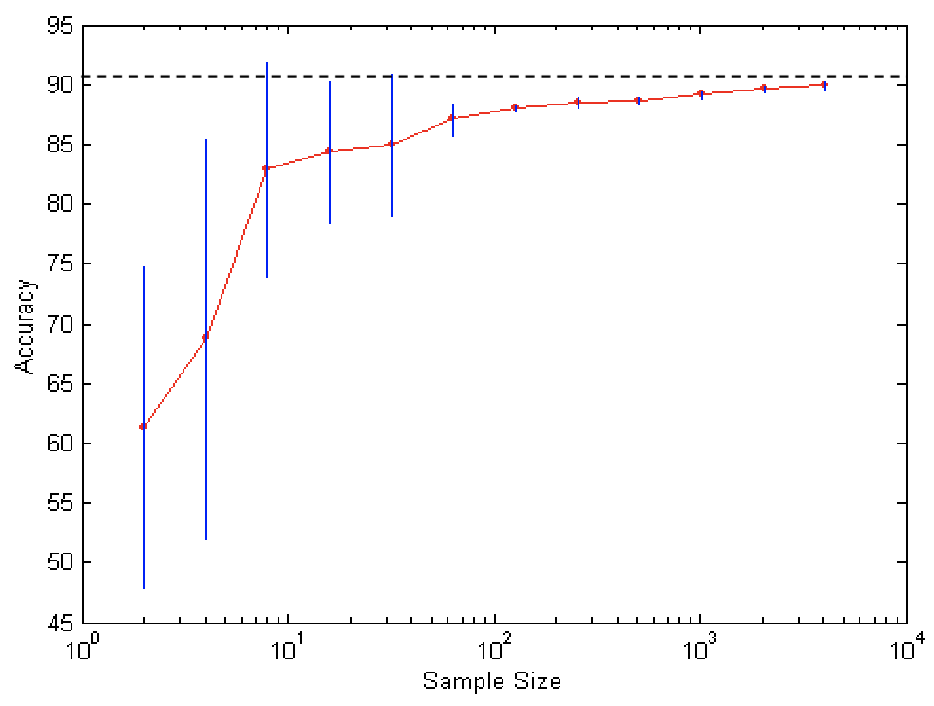
\includegraphics[width=0.5\linewidth]{img/Learning curve.png}
    \caption{The learning curve plotted for different sizes of the training dataset.}
\end{figure}
In the figure above, we may choose $10^2$ as the ideal size of the dataset. This method needs caution, since s sample size too small may show bias in the data represented or too much variance in the estimate.

There are many techniques for model assessment and evaluation, such as holdout, random subsampling (randomized repeated holdout), cross validation, stratified sampling, bootstrap, etc. (SEE ML NOTES).

\textbf{Holdout} is simple, but uses only part of the data for training and part for testing. Repeated holdout performs holdout multiple times by choosing the test set randomly each time, and the final estimation is the mean across all evaluations. This approach is still not optimal, since the test set of one iteration may overlap with the test set of another.

A better technique is \textbf{K-fold cross validation}. The dataset is partitioned into $K$ parts; then, for each value of $K$, the $K^{th}$ part is taken as the validation/test set, while the rest is the training/training + validation set. Often, it is used in conjunction with stratification to make sure that each part represents the target classes equally. After performing the validation/testing on all $K$ parts, the error is calculated as the average across all folds. This provides a better estimate than simple holdout methods.

\subsection{Methods for Model Comparison}

\subsubsection{ROC Curve}

Assessing the performance of a classifier over a range of score thresholds is called \textbf{aggregate evaluation} of performance. One of the widely used tools for aggregate evaluation is the \textbf{Receiver Operating Characteristic (ROC) curve}. A ROC curve is a graphical approach to visualize the trade off between TPR (true positive rate, plotted in the y axis) and FPR (false positive rate, plotted on the x axis) of a classifier. It shows he ability of a binary classifier as the discrimination threshold is varied, so each point corresponds to a different threshold value.

The following procedure describes the generic approach for computing a ROC curve:

\begin{enumerate}
    \item Sort the test instances in increasing order of their scores (can be posterior probability calculated using some other classifier).

    \item Select the lowest ranked test instance (with the lowest score), and assign that instance and all the ones ranked higher to the positive class. Since all the positive instances are classified correctly and all negative one are misclassified, $\textit{TPR} = \textit{FPR} = 1$.

    \item Select the next test instance from the list. Classify the selected instance and those ranked higher as positive, anything below as negative. Update TP and FP counts accordingly.

    \item Repeat the previous step and update TP and FP counts until the highest ranked instance is selected. At this final stage, $\textit{TPR} = \textit{FPR} = 0$.

    \item Plot the TPR against the FPR.
\end{enumerate}

A perfect model with 0 misclassifications would have $\textit{FPR} = 0$ and $\textit{TPR} = 1$. To summarize the aggregate behaviour across all operating points, one of the most commonly used measures is the \textbf{area under the ROC curve (AUC)}. If the classifier is perfect, the AUC is equal to 1. If the classifier is bad, and behaves as a random guesser, the AUC will be 0.5.

Note that when comparing different models using AUC, we cannot say that a model is better than another for simply having an higher AUC (unless the difference is drastic enough). Consider the ROC curves for the models $M_1$ and $M_2$ pictured below:

\begin{figure}[h]
    \centering
    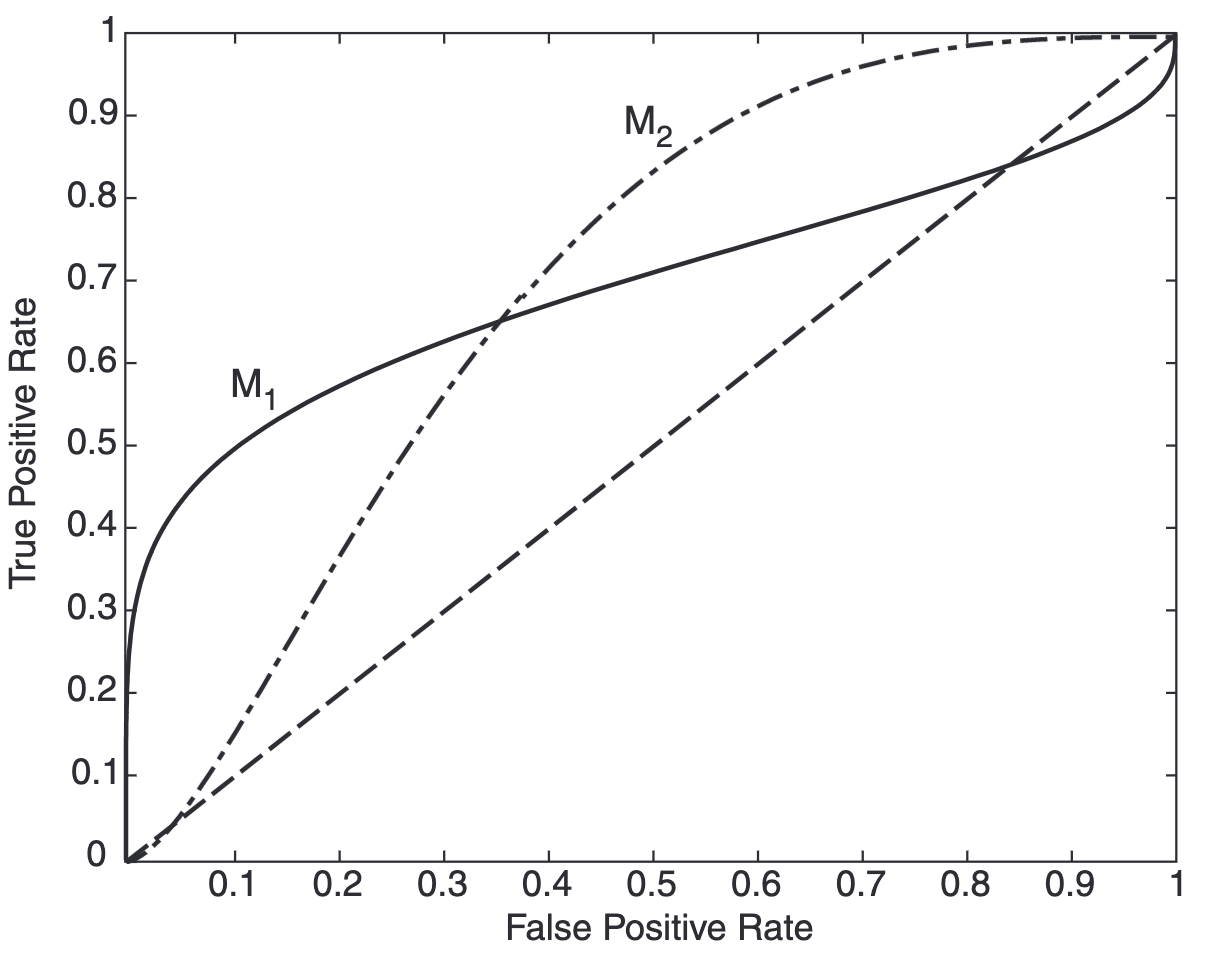
\includegraphics[width=0.5\linewidth]{img/ROC_comparison.png}
    \caption{ROC curves for two different classifiers.}
\end{figure}

$M_2$ does have a slightly bigger AUC compared to $M_1$, but they are both good at different things: $M_1$ is better for small FPR, while $M_2$ is better for large FPR.

\subsubsection{Lift Chart}

The \textbf{lift chart} (or \textbf{gains chart}) is another popular technique, used often in direct marketing. The input is a dataset where each ``case'' is scored with the estimated probability that it will belong to a given class. The lift chart is the constructed by plotting the cumulative number of cases (on the x axis) against the cumulative number of true positives (on the y-axis). 

\begin{figure}[h]
    \centering
    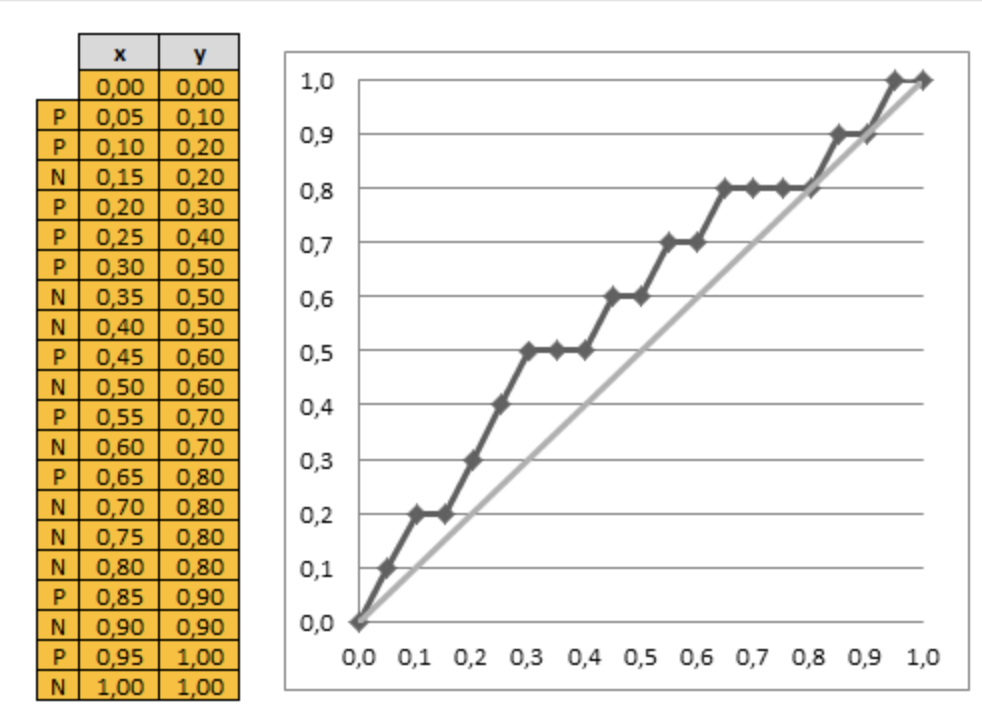
\includegraphics[width=0.5\linewidth]{img/Lift chart.png}
    \caption{Example of lift chart.}
\end{figure}

The gray line is a reference line. For any given number of cases, it represents the expected number of positives we would predict if we did not have a model, but simply selected at random (similarly to the line in the middle of the ROC curve plot).

From this chart, we can derive an economical value plot; e.g., given a predictive model for target marketing, how many customers should we target to maximize income? The profit is given by the following formula: $\textit{UnitB} * \textit{MaxR} * \textit{Lift}(X) - \textit{UnitCost}*N*X/100$, where \textit{UnitB} is the unit benefit, \textit{MaxR} is the expected number of potential responders in the population considered (of size $N$), $\textit{Lift}(X)$ is the lift chart value for $X \in [0,1]$, and \textit{UnitCost} is the unit postal cost.

\begin{figure}
    \centering
    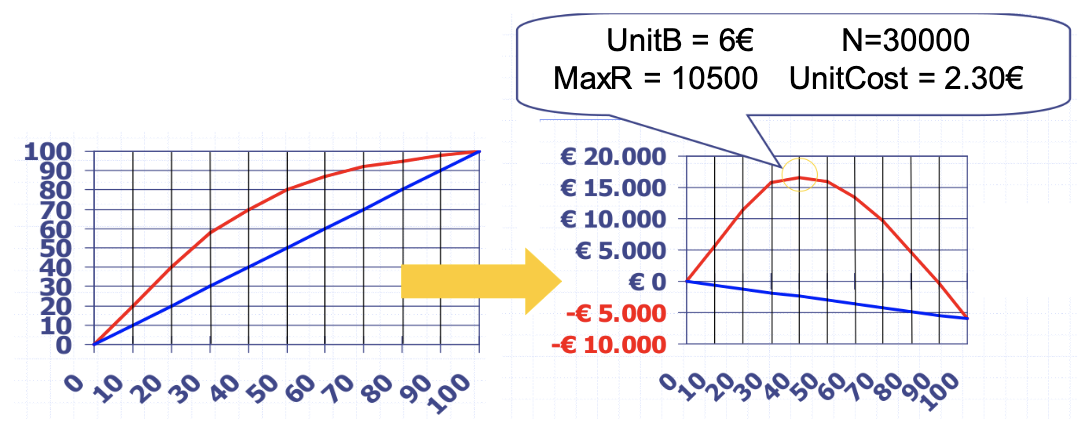
\includegraphics[width=0.5\linewidth]{img/Lift chart application.png}
    \caption{Example of application of a lift chart.}
\end{figure}


\section{Issues of Classification}

\subsection{Underfitting and Overfitting}

As of now, we considered algorithms that construct models with the lowest possible training error. In practice, however, if a model fits the data too much, it incurs into \textbf{overfitting}. Overfitting happens when the training error is very low, but the generalization error is high. This means that the model is too adapted to the training data (also said to be ``overtrained''), and cannot accurately predict unseen instances. \textbf{Underfitting} is the opposite phenomenon, when the model is not adapted enough to the training data, thus producing an also high generalization error. These phenomenons are controlled by the \textbf{complexity} of the model. Each model has a different way to measure this complexity. In the case of a K-NN classifier, the complexity is inversely proportional to the number of neighbors that make a neighborhood. For decision trees, the complexity is proportional to the depth of the tree.

Another problem that can cause overfitting regardless of the training/validation procedure is the lack of sufficient training examples. The likelihood of incurring into overfitting is inversely proportional to the number of the available training instances. 

\textbf{The course slides seem to imply that overfitting can be caused by the mere presence of noisy data. This is inexact; overfitting is caused by having a model so complex it adapts too much to noisy data, but the presence itself of noise should not be a concern given appropriate regularization.}

\subsection{Model Selection}

Model selection is the phase in which the model's parameters and hyperparameters are chosen. This is done by using a training set along with a \textbf{validation} set (containing instances selected from the training set). The model is first set up with some starting values of parameters and hyperparameters. The model is trained on the training set, and the generalization error is estimated by the error calculated on the validation set. After a model with an acceptable validation error is selected, its quality is assessed using the test set instances.

There's many ways to divide the data to perform training, validation, and testing. The simplest way is \textbf{hold-out}, in which the training set is split into three partitions, one for testing, one for validation, and one for testing. This technique, however, ``wastes'' the data as only some of it can be used for each step. Another technique is \textbf{k-fold cross validation} (it can be used for testing as well, either in combination with hold-out, or with cross-validation). The dataset $D$ is split into $k$ partitions; then, for each partition $D_i$, training is done using $D / D_i$, and validation is performed using $D_i$ only. This way, testing and validation is repeated multiple times with different data, obtaining a more accurate estimation of the generalization error.

To select the final model, the strategy used is inspired by \textbf{Occam's razor/principle of parsimony}: when presented with two models with the same errors, the simpler model is preferred over the more complex one; again, we prefer simpler models because they're less likely to fall into overfitting. One way to estimate the generalization error of the model is:

\begin{equation*}
    R(\textit{Model}) = R_{emp}(\textit{Model}, \textit{TR}) + \alpha \textit{Complexity}(\textit{Model})
\end{equation*}

\subsection{Model Assessment}

There's three ways to estimate the generalization error:
\begin{itemize}
    \item \textbf{Pessimistic estimate}: the generalization error rate is assumed to be worse than the training error rate;
    \item \textbf{Optimistic/resubstitution estimate}: the generalization error rate is assumed to be the same as the training error rate;
    \item \textbf{Reduced error pruning (REP)}: the generalization error rate is assumed to be the same as the validation error rate.
\end{itemize}

Let's consider error estimation for decision tree classifiers. The pessimistic error estimate for a decision tree $T$ with $k$ leaf nodes is:

\begin{equation*}
    R(T) = R_{emp}(T) + \omega \dfrac{k}{N_{train}} \,,
\end{equation*}
where $\omega$ is the cost of adding a leaf node, and $N_{train}$ is the number of training instances. The optimistic error estimation would simply be:
\begin{equation*}
    R(T) = R_{emp}(T)
\end{equation*}

\subsection{Addressing Overfitting in Decision Trees}

A common regularization technique used for decision trees is \textbf{pre-pruning}, which is a form of early stopping. The training algorithm is stopped before the tree is fully formed, without necessarily having all leaf nodes with instances of one class only. We can set new conditions such as:
\begin{itemize}
    \item the number of instances is less than some user-defined threshold;
    \item the class distribution of instances is independent from the available features (e.g. tested using a $\chi^2$ test);
    \item the current node does not improve impurity measures;
    \item the estimated generalization error falls below a certain acceptable threshold.
\end{itemize}

Alternatively, we can employ \textbf{post-pruning}. The decision tree is grown in its entirety; then, nodes are trimmed from the bottom. If a trimming improves the generalization error, it's accepted, replacing the pruned subtree with a single leaf. The label corresponding to the leaf is chosen as the majority class of instances in the subtree.
